\chapter{pgfplots}

pgfplots 是一個可以畫出複雜的三維圖表的強大 Package,需要注意的是這個 Package 是基於前面介紹過的 \TikZ\ ,所以在使用之前請記得要先使用 \TikZ 。

\section{簡介}

在使用 pgfplots 之前我們需要先使用 tikzpicture 環境,之後再使用 pgfplots  提供的 axis 環境。

\begin{tcblisting}{}
\begin{tikzpicture}
\begin{axis}
......
\end{axis}
\end{tikzpicture}
\end{tcblisting}

我們要將 pgfplots 提供的命令放在 axis 環境中,第一個要介紹的是  \verb`\addplot` 這個命令,大部分可選參數是與 \TikZ 的可選參數相同,方程式則是與大部分程式語言的表達方式一樣。

\begin{tcblisting}{}
%\addplot[可選參數]{方程式}
\begin{tikzpicture}
\begin{axis}
\addplot[domain=-5:5, color=blue] {x^2};
\end{axis}
\end{tikzpicture}
\end{tcblisting}

使用完之後也請不要忘記在最後面加上 ;。

\section{二維圖形}

\subsection{函數圖}

第一個介紹的還是函數圖,簡單的範例上面展示過了,所以這裡會比較注重在介紹不同的可選參數。

\begin{tcblisting}{}
\begin{tikzpicture}
\begin{axis}
\addplot[domain=-5:5, color=blue] {x^2};
\end{axis}
\end{tikzpicture}
\end{tcblisting}

這是上面所展示的陽春例子,我們可以再多加一個方程式讓他看起來好一點。

\begin{tcblisting}{}
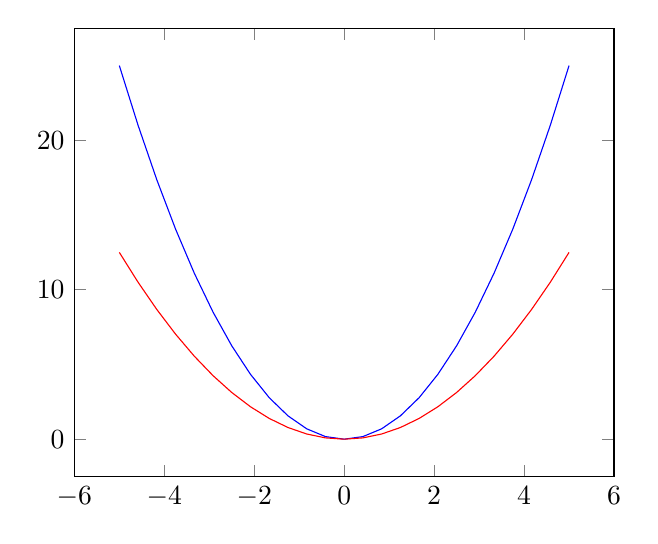
\begin{tikzpicture}
\begin{axis}
\addplot[domain=-5:5, color=blue] {x^2};
\addplot[domain=-5:5, color=red] {x^2/2};
\end{axis}
\end{tikzpicture}
\end{tcblisting}

可是這樣沒有標示難免會讓人搞混,所以我們可以利用 \verb`\addlegendentry ` 加入註解。

\begin{tcblisting}{}
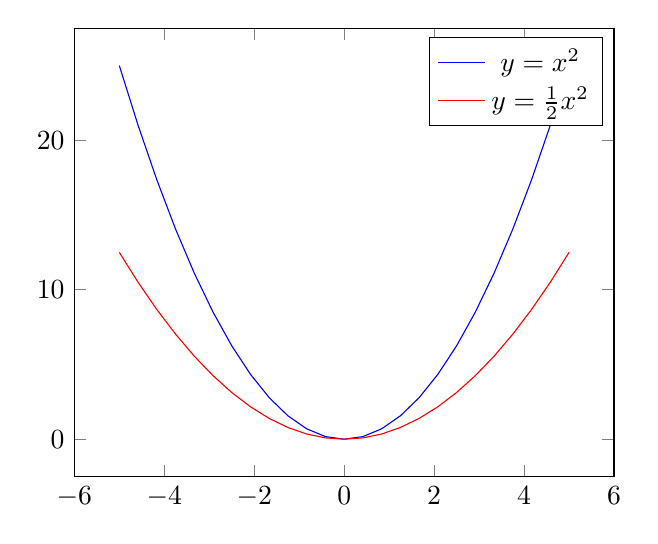
\begin{tikzpicture}
\begin{axis}
\addplot[domain=-5:5, color=blue] {x^2};
\addlegendentry{\(y=x^2\)}
\addplot[domain=-5:5, color=red] {x^2/2};
\addlegendentry{\(y=\frac{1}{2}x^2\)}
\end{axis}
\end{tikzpicture}
\end{tcblisting}

這樣就不會搞混了,如果今天想要用對數來當 x, y 軸的單位,pgfplots 也有提供 \verb`\begin{semilogxaxis}` 與 \verb`\begin{semilogyaxis}` 來解決這個問題。

\begin{tcblisting}{}
\begin{tikzpicture}
\begin{semilogyaxis}
\addplot[domain=-10:10, color=blue, samples=1000] {log10(x)};
\end{semilogyaxis}
\end{tikzpicture}
\end{tcblisting}

有時候座標軸會不符合我們想要的樣式,這時可以利用 axis lines 來調整。

\begin{tcblisting}{}
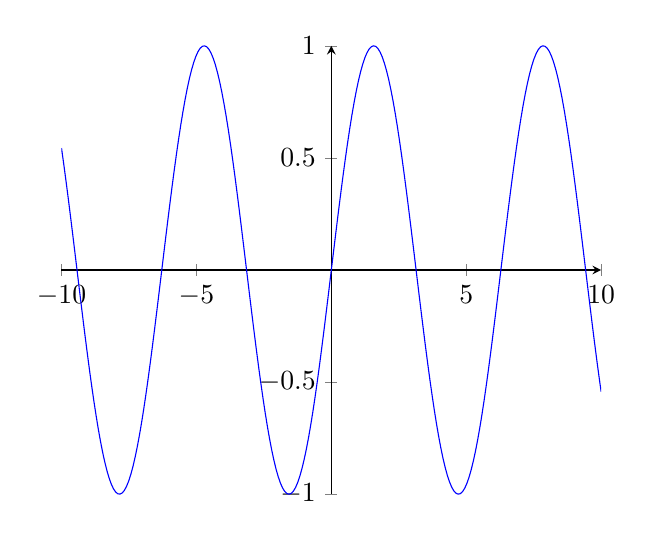
\begin{tikzpicture}
\begin{axis}[axis lines = middle]
\addplot[domain=-10:10, color=blue, samples=250] {sin(deg(x))};
\end{axis}
\end{tikzpicture}
\end{tcblisting}

\subsection{折線圖}

除了函數圖外,pgfplots 也可以繪製折線圖。

\begin{tcblisting}{}
\begin{tikzpicture}
\begin{axis}
\addplot coordinates{(0,0)(1,4)(2,3)(3,5)(4,2)(5,1)(6,0)(7,8)};
\end{axis}
\end{tikzpicture}
\end{tcblisting}

在 coordinates 後面的將放入所有折線圖的點,就可以畫出折線圖了,但有時座標軸上的標記與想像中的並不一樣,這時就需要用 xtick 與 ytick 調整。

\begin{tcblisting}{}
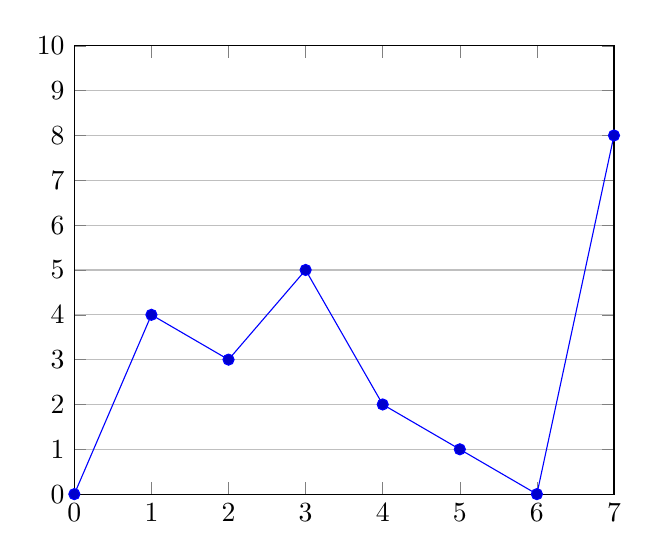
\begin{tikzpicture}
\begin{axis}[
xmin=0, xmax=7,
ymin=0, ymax=10,
xtick={0,1,2,3,4,5,6,7},
ytick={0,1,2,3,4,5,6,7,8,9,10},
ymajorgrids=true,
]
\addplot coordinates{(0,0)(1,4)(2,3)(3,5)(4,2)(5,1)(6,0)(7,8)};
\end{axis}
\end{tikzpicture}
\end{tcblisting}

\begin{itemize}
\item xmin, ymin, xmax, ymax 這些是指定 x 軸與 y 軸的最大、最小值
\item xtick, ytick 是指定 x 軸與 y 軸上的標記的位置
\item ymajorgrids 是繪製出與 y 軸相交的格線,可以用 xmajorgrids 來繪製出與 x 軸相交的格線,或用 grids=major 同時繪製兩者。
\end{itemize}

\subsection{長條圖}

長條圖與折線圖有者異曲同工之妙

\begin{tcblisting}{}
\begin{tikzpicture}
\begin{axis}[ybar, ybar interval=0.75, enlargelimits=0.1]
\addplot coordinates{(2040,9.50)(2030,10.60) (2020,12.58)};
\addplot coordinates{(2020,17.50) (2030,24.10) (2040,30.60)};
\legend{0~14歲人口所占比率(\%),65歲以上人口所占比率(\%)}
\end{axis}
\end{tikzpicture}
\end{tcblisting}

\begin{itemize}
\item ybar 指的是長條與 y 軸平行,另外還有 xbar 這個選項可以用。
\item ybar interval 是指定長條之間的空隙,1 代表沒有空隙。
\item enlarge limits 是調整整個座標軸與圖表的元素間的距離,另外也可以用enlarge x limits, enlarge y limits 等等來單獨調整特定的座標軸。
\end{itemize}

\subsection{散佈圖}

散佈圖也很簡單。

\begin{tcblisting}{}
\begin{tikzpicture}
\begin{axis}
\addplot[scatter, mark=*, only marks]
coordinates{(143,62) (50,594) (165,53) (139,348) (145,194) (75,533) (51,258) (154,492)};
\end{axis}
\end{tikzpicture}
\end{tcblisting}

\begin{itemize}
\item scatter 是讓顏色依據 y 軸的數值而變化
\item only marks 是不讓點之間用線連起來
\item mark 是指定點的標記的樣式
\end{itemize}

\subsection{從其他檔案輸入數據}

上面的方法這只適用於數據只有寥寥幾筆時,不然如果有一千多筆,一個一個 key 未免太過勞神費力,不過 pgfplots 都幫你想好了,他可以讓你從 .dat 或 .csv 檔中輸入數據。

\begin{tcblisting}{}
\begin{tikzpicture}
\begin{axis}[x tick label style={/pgf/number format/1000 sep=},width=10cm, grid=major]
\addplot table [x=year, y=youth, col sep=comma, mark=none] {data.csv};
\addlegendentry{0~14歲人口所占比率(%)}
\addplot table [x=year, y=old, col sep=comma, mark=none] {data.csv};
\addlegendentry{65歲以上人口所占比率(%)}
\end{axis}
\end{tikzpicture}
\end{tcblisting}

\begin{itemize}
\item x tick label style 是調整 x 軸上標示的樣式。
\item table 是表示資料來源是類似表格的形式。
\item x=, y= 是指定 x, y 的數據要從哪一欄輸入。
\item col sep 是告訴 pgfplots 欄與欄的分界是用什麼符號。
\end{itemize}

\section{三維圖形}

終於進入三維圖形了,三維圖形的繪製方式與二維圖形相似,只是命令要改用 \verb`\addplot3` 這個命令外,其他的選項幾乎都通用。

\begin{tcblisting}{}
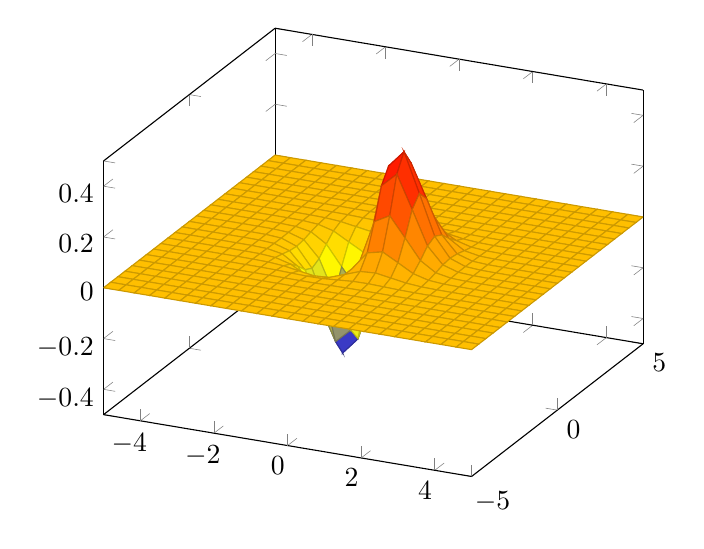
\begin{tikzpicture}
\begin{axis}
\addplot3[surf] {exp(-x^2-y^2)*x};
\end{axis}
\end{tikzpicture}
\end{tcblisting}

surf 是 surface 的縮寫與 scatter 有異曲同工之妙,同樣會因為某一軸的數值高低而產生顏色變化。